





XtreemFS uses ONC RPC\cite{RFC1831}\index{ONC RPC} for executing remote operations. Interfaces and records are defined in a subset of CORBA IDL\index{IDL}. Yidl\footnote{http://code.google.com/p/yield/} is used to generate the code for the interfaces and records in C++ and Java.

To build the Java classes from the interfaces:
\begin{enumerate}
 \item export \texttt{PYTHONPATH} to point to your yidl source directory:\\
       \texttt{export PYTHONPATH=/home/user/yidl/src}
 \item execute \texttt{bin/generate\_xtreemfs\_java.py}
\end{enumerate}


\makeatletter
\renewcommand\paragraph{\@startsection{paragraph}{4}{\z@}%
  {-3.25ex\@plus -1ex \@minus -.2ex}%
  {0.1ex \@plus .0ex}%
  {\normalfont\normalsize\bfseries}}
\makeatother

\subsection{Constants}
\label{sec:xtreemfs_proto_const}

Globally shared constants are defined in \texttt{in\-ter\-faces/const\-ants.idl}.

\begin{description}
	\item[\texttt{ACCESS\_CONTROL\_POLICY\_NULL}] don't use any access policy (on the MRC\index{MRC}). This will allow all users to do everything on the volume.

	\item[\texttt{ACCESS\_CONTROL\_POLICY\_POSIX}] use standard POSIX\index{POSIX} permissions (user, group, others) on the volume.

	\item[\texttt{ACCESS\_CONTROL\_POLICY\_VOLUME}] similar to POSIX\index{POSIX} permissions but the permission for the root (/) is used for the entire volume.

	\item[\texttt{ACCESS\_CONTROL\_POLICY\_DEFAULT}] the policy to use in e.g. mkvol if nothing is specified.

	\item[\texttt{ONCRPC\_SCHEME}] scheme for URLs.

	\item[\texttt{ONCRPCS\_SCHEME}] scheme for URLs when using SSL.

	\item[\texttt{ONCRPC\_AUTH\_FLAVOR}] constant to use for ONC RPC\index{ONC RPC} auth\_flavor to indicate XtreemFS auth. If present, a UserCredentials record is sent in auth\_opaque

	\item[\texttt{OSD\_SELECTION\_POLICY\_SIMPLE}] only OSDs which are alive and which have more than 2GB free space are used.

	\item[\texttt{OSD\_SELECTION\_POLICY\_DEFAULT}] the policy to use in e.g. mkvol if nothing is specified.

	\item[\texttt{REPL\_UPDATE\_PC\_NONE}] no replication is used

	\item[\texttt{REPL\_UPDATE\_PC\_RONLY}] read-only replication

	\item[\texttt{SERVICE\_TYPE\_MRC}] for DIR\index{DIR} service registry, service is an MRC\index{MRC}

	\item[\texttt{SERVICE\_TYPE\_OSD}] for DIR\index{DIR} service registry, service is an OSD\index{OSD}

	\item[\texttt{SERVICE\_TYPE\_VOLUME}] for DIR\index{DIR} service registry, service is a volume

	\item[\texttt{STRIPING\_POLICY\_RAID0}] RAID0 (striping)

	\item[\texttt{STRIPING\_POLICY\_DEFAULT}] the policy to use in e.g. mkvol if nothing is specified.

	\item[\texttt{STRIPING\_POLICY\_STRIPE\_SIZE\_DEFAULT}] default stripe size in KB to use if nothing is specified.

	\item[\texttt{STRIPING\_POLICY\_WIDTH\_DEFAULT}] default striping width (number of OSDs\index{OSD}) to use if nothing is specified.

	\item[\texttt{SYSTEM\_V\_FCNTL\_H\_O\_...}] POSIX\index{POSIX} constants

\end{description}

\subsection{Types}

\subsubsection{Globally Shared Types}

Globally shared data structures are defined in \texttt{inter\-faces/types.idl}.

\paragraph{\texttt{struct UserCredentials}}

User information sent in the ONC RPC\index{ONC RPC} \texttt{opaque\_auth} body if XtreemFS authentication is used. How the userID and groupIDs look like depends on the policy used in the client which translates the local uid/gid.

\begin{tabularx}{\textwidth}{lX}
 \texttt{user\_id} & globally unique userID\\
 \texttt{group\_ids} & list of globally unique groupIDs (must contain at least one entry)\\
 \texttt{password} & admin password (in cleartext) required for some operations (e.g. mkvol)
\end{tabularx}

\paragraph{\texttt{struct VivaldiCoordinates}}

Structure used to exchange Vivaldi coordinates between components, also used in UDP\index{UDP} packets for measuring latency between XtreemFS clients and OSDs\index{OSD}.

\begin{tabularx}{\textwidth}{lX}
 \texttt{x\_coordinate} & x coordinate\\
 \texttt{y\_coordinate} & y coordinate\\
 \texttt{local\_error} & confidence in correctness of x/y coordinates
\end{tabularx}


\subsubsection{Types Shared between MRC\index{MRC} and OSD\index{OSD}}

Types that are mainly shared between MRC\index{MRC} and OSD\index{OSD} are defined in \texttt{inter\-faces/mrc\_osd\_\-types.idl}.

\paragraph{\texttt{struct NewFileSize}}
Sent by the OSD\index{OSD} in response to a file modification operation if the file size has changed. A client may cache these updates and send them to the MRC\index{MRC} when renewing a capability, on fsync/flush and close. The client needs only to send the most recent record it received from the OSD\index{OSD} for a given file. Most recent means that: \texttt{
(size\_in\_bytes' $>$ size\_in\_bytes} \texttt{AND} \texttt{truncate\_epoch' == truncate\_epoch) 
OR} \texttt{(truncate\_epoch' $>$ truncate\_epoch)}

The client should update its local file size cache with the NewFileSize records received from the OSD\index{OSD}. The client should use the \textit{locally cached} file size on stat rather than the result from the MRC\index{MRC} to ensure that local processes see their own modifications.

\begin{tabularx}{\textwidth}{lX}
 \texttt{size\_in\_bytes} & the new file size in bytes\\
 \texttt{truncate\_epoch} & truncate epoch in which this operation was executed (used by the MRC\index{MRC} for ordering updates)
\end{tabularx}


\paragraph{\texttt{struct OSDtoMRCData}}
Data sent by the OSD\index{OSD} to the client which is expected to pass it on to the MRC\index{MRC}. When the data should be passed to the MRC\index{MRC} depends on the \texttt{caching\_policy}. This feature is currently not used.

\begin{tabularx}{\textwidth}{lX}
 \texttt{caching\_policy} & describes how the client is allowed to cache the data (when to send it to the MRC\index{MRC})\\
 \texttt{data} & opaque data
\end{tabularx}

\paragraph{\texttt{struct OSDWriteResponse}}
Record containing file size updates and/or OSDtoMRCData. Returned from all data-modifying operations.

\begin{tabularx}{\textwidth}{lX}
 \texttt{new\_file\_size} & contains no record or at most one record if the file size changed\\
 \texttt{opaque\_data} & contains 0 or more records
\end{tabularx}


\paragraph{\texttt{struct StripingPolicy}}
Describes how a replica (one copy of the file) is split into objects.

\begin{tabularx}{\textwidth}{lX}
 \texttt{policy} & describes the scheme to use for distributing the objects among the OSDs\index{OSD}, e.g. RAID0 for simple round robin striping.\\
 \texttt{stripe\_size} & the size of the objects in kilobytes, must be $>= 4$\\
 \texttt{width} & the number of OSDs\index{OSD} to use for striping, must be $>= 1$.
\end{tabularx}


\paragraph{\texttt{struct Replica}}
Describes a single copy of a file.

\begin{tabularx}{\textwidth}{lX}
 \texttt{striping\_policy} & the striping policy to use for this replica.\\
 \texttt{replication\_flags} & value depends on the replication policy, e.g. to indicate a full or lazy replica.\\
 \texttt{osd\_uuids} & ordered (!) list of OSDs\index{OSD} holding objects of the file.
\end{tabularx}



\paragraph{\texttt{struct XLocSet}}
Describes a complete file together with all replicas (copies) and how they are kept consistent.

\begin{tabularx}{\textwidth}{lX}
 \texttt{replicas} & list of the file's replicas (i.e. list of Replica structs)\\
 \texttt{version} & incremented by the MRC\index{MRC} on each modification of the list. Used by the OSD\index{OSD} to reject clients working with outdated lists.\\
 \texttt{repUpdatePolicy} & the policy used for keeping replicas in sync. \\
 \texttt{read\_only\_file\_size} & the size of the file in bytes, used only for read-only replication.
\end{tabularx}


\paragraph{\texttt{struct XCap}}
Security token which is issued by the MRC\index{MRC} and authorizes a client to execute operations on a file at the OSDs\index{OSD}.

\begin{tabularx}{\textwidth}{lX}
 \texttt{file\_id} & file for which the capability can be used\\
 \texttt{access\_mode} & POSIX\index{POSIX} access mode for which client is authorized (e.g. read only, delete, write, truncate).\\
 \texttt{expires\_s} & absolute timestamp when the capability becomes invalid (seconds since epoch). \\
 \texttt{client\_identity} & the client identity set by the MRC\index{MRC}, currently the client's IP address. \\
 \texttt{truncate\_epoch} & the file's current truncate epoch. \\
 \texttt{server\_signature} & the MRC's\index{MRC} signature for the capability which is used by the OSD\index{OSD} to validate the XCap. Signature is created using shared secret specified in the MRC\index{MRC} and OSD\index{OSD} configuration. \\
\end{tabularx}



\paragraph{\texttt{struct FileCredentials}}
A record containing the XLocSet and XCap for a file. Required for most OSD\index{OSD} operations.

\begin{tabularx}{\textwidth}{lX}
 \texttt{xlocs} & the XLocSet\\
 \texttt{xcap} & the capability\\
\end{tabularx}


\paragraph{\texttt{sequence<FileCredentials> FileCredentialsSet}}
Used by the MRC\index{MRC} to return no or at most one FileCredentials record.





% %%%%%%%%%%%%%%%%%%%%%%%%%% EXCEPTIONS %%%%%%%%%%%%%%%%%%%%%%%%%%%%%%%%%
\subsubsection{Exceptions}

Exceptions that may be thrown in connection with an RPC are defined in \texttt{interfaces/exceptions.idl}.

\paragraph{\texttt{exception ProtocolException}}
Thrown on ONC RPC\index{ONC RPC} errors (e.g. GARBAGE\_ARGS)

\begin{tabularx}{\textwidth}{lX}
 \texttt{accept\_stat} & ONC RPC\index{ONC RPC} \texttt{accept\_stat} value\\
 \texttt{error\_code} & POSIX\index{POSIX} errno, if available\\
 \texttt{stack\_trace} & optional, for debugging only
\end{tabularx}


\paragraph{\texttt{exception errnoException}}
Thrown by the MRC\index{MRC} to indicate a POSIX\index{POSIX} error.

\begin{tabularx}{\textwidth}{lX}
 \texttt{error\_code} & POSIX\index{POSIX} errno, if available\\
 \texttt{error\_message} & optional text message\\
 \texttt{stack\_trace} & optional, for debugging only
\end{tabularx}


\paragraph{\texttt{exception RedirectException}}
Thrown by the DIR\index{DIR},MRC\index{MRC} and OSD\index{OSD} to redirect the client to another service. Use e.g. for master slave replication to direct the client to the current master.

\begin{tabularx}{\textwidth}{lX}
 \texttt{to\_uuid} & service to contact\\
\end{tabularx}


\paragraph{\texttt{exception ConcurrentModificationException}}
Thrown by the DIR\index{DIR} if a record was modified by another service on the meantime.

\begin{tabularx}{\textwidth}{lX}
 \texttt{stack\_trace} & optional, for debugging only
\end{tabularx}


\paragraph{\texttt{exception InvalidArgumentException}}
Thrown by the DIR\index{DIR} if an input value is not acceptable.

\begin{tabularx}{\textwidth}{lX}
 \texttt{error\_message} & error message describing the correct values.
\end{tabularx}


% %%%%%%%%%%%%%%%%%%%%%%%%%% DIR INTERFACE %%%%%%%%%%%%%%%%%%%%%%%%%%%%%%%%%
\subsection{Directory Service Interface}

The Directory Service interface is defined in \texttt{interfaces/dir\_interface.idl}.

\paragraph{\texttt{struct AddressMapping}}
Maps a service UUID to protocol, hostname/IP and port. A service can have multiple mappings for different networks (e.g. inside a cluster with private IP addresses). At the moment only ``*'' is supported for \texttt{match\_network} which indicates a match for all networks.

\begin{tabularx}{\textwidth}{lX}
 \texttt{uuid} & the service UUID\\
 \texttt{version} & the record's version, used by the DIR\index{DIR} to detect concurrent modifications\\
 \texttt{protocol} & the protocol used by the service\\
 \texttt{address} & resolvable hostname or IP address in text form\\
 \texttt{port} & port on which the service listens\\
 \texttt{match\_network} & for future use, must be \texttt{*}\\
 \texttt{ttl\_s} & time to live in seconds, indicates how long this record can be cached before it is re-fetched from the DIR\index{DIR}\\
\end{tabularx}

\paragraph{\texttt{sequence<AddressMapping> AddressMappingSet}}
Future releases of XtreemFS will support multi-network setups to ease the usage of XtreemFS in shared public/private network environments often found in clusters.


\paragraph{\texttt{struct Service}}
Information on a service registered at the DIR\index{DIR}.

\begin{tabularx}{\textwidth}{lX}
 \texttt{uuid} & the service UUID\\
 \texttt{version} & the record's version, used by the DIR\index{DIR} to detect concurrent modifications\\
 \texttt{type} & service type (see \ref{sec:xtreemfs_proto_const})\\
 \texttt{name} & human readable name of the service; for volumes: the unique volume name\\
 \texttt{last\_updated\_s} & timestamp of the last time (in seconds since epoch) the service updated its entry at the DIR\index{DIR}. Used as a coarse-grained heartbeat-signal.\\
 \texttt{data} & a map of additional data which depends on the service (e.g. MRC\index{MRC} of a volume or free space of an OSD\index{OSD})\\
\end{tabularx}


\paragraph{\texttt{void xtreemfs\_address\_mappings\_get( string uuid, out AddressMappingSet address\_mappings~)}}
Get an address mapping for the service specified by \texttt{uuid}.

\begin{tabularx}{\textwidth}{lX}
 \texttt{uuid} & the service UUID\\
 \texttt{out address\_mappings} & empty, if no mapping exists, one (or more) records otherwise\\
\end{tabularx}


\paragraph{\texttt{void xtreemfs\_address\_mappings\_remove( string uuid~)}}
Remove an address mapping from the DIR\index{DIR}.

\begin{tabularx}{\textwidth}{lX}
 \texttt{uuid} & the service UUID\\
\end{tabularx}


\paragraph{\texttt{uint64\_t xtreemfs\_address\_mappings\_set( AddressMappingSet address\_mappings~)}}
Updates the address mappings for a service. 

\begin{tabularx}{\textwidth}{lX}
 \texttt{address\_mappings} & the new mappings. The UUID in all records must be the same. The version must be 0 for a new mapping or the version obtained with the last read from the DIR\index{DIR}.\\
 returns & the new version of the mapping\\
 throws & ConcurrentModificationException if the record was updated (version incremented by DIR\index{DIR}) between reading and updating the record.
\end{tabularx}


\paragraph{\texttt{void xtreemfs\_checkpoint()}}
Forces the DIR\index{DIR} to create a BabuDB checkpoint. This operation does not block, the checkpoint is created asynchronously. The admin password must be sent via the XtreemFS authentication.


\paragraph{\texttt{uint64\_t xtreemfs\_global\_time\_s\_get()}}
Returns the current system time on the DIR\index{DIR} in seconds since epoch. Used to synchronize MRCs\index{MRC} and OSDs\index{OSD} to the global XtreemFS system time. The DIR\index{DIR} system should be synchronized with a precise clock using e.g. ntp.

\begin{tabularx}{\textwidth}{lX}
 returns & system time in seconds since UNIX epoch.
\end{tabularx}


\paragraph{\texttt{void xtreemfs\_service\_get\_by\_type( uint16\_t type, out ServiceSet services~)}}
Get all services of a specific type registered at the DIR\index{DIR}.

\begin{tabularx}{\textwidth}{lX}
 \texttt{type} & the service type to return\\
 \texttt{out services} & all matching services\\
\end{tabularx}


\paragraph{\texttt{void xtreemfs\_service\_get\_by\_uuid( string uuid, out ServiceSet services~)}}
Get the service information for a service with a specific UUID.

\begin{tabularx}{\textwidth}{lX}
 \texttt{uuid} & the service uuid\\
 \texttt{out services} & one record, if the service is registered, empty list otherwise\\
\end{tabularx}


\paragraph{\texttt{void xtreemfs\_service\_get\_by\_name( string name, out ServiceSet services~)}}
Get the service information for a service with a specific name.

\begin{tabularx}{\textwidth}{lX}
 \texttt{name} & the service's name\\
 \texttt{out services} & one record, if the service is registered, empty list otherwise\\
\end{tabularx}



\paragraph{\texttt{uint64\_t xtreemfs\_service\_register( Service service~)}}
Update a service registration at the DIR\index{DIR}. Updates the \texttt{last\_update\_s} field of the service.

\begin{tabularx}{\textwidth}{lX}
 \texttt{service} & the service's data. The UUID must be the service's UUID, the version must be 0 for a new service or the version obtained with the last read from the DIR\index{DIR}.\\
 returns & the new version of the mapping\\
 throws & ConcurrentModificationException if the record was updated (version incremented by DIR\index{DIR}) between reading and updating the record.\\
\end{tabularx}


\paragraph{\texttt{void xtreemfs\_service\_deregister( string uuid~)}}
Removes the service registry entry for the service from the DIR\index{DIR}.

\begin{tabularx}{\textwidth}{lX}
 \texttt{uuid} & the service uuid\\
\end{tabularx}


\paragraph{\texttt{void xtreemfs\_service\_offline( string uuid~)}}
Sets the \texttt{last\_update\_s} field to 0 which indicates that the service was taken offline.

\begin{tabularx}{\textwidth}{lX}
 \texttt{uuid} & the service uuid\\
\end{tabularx}


\paragraph{\texttt{void xtreemfs\_shutdown()}}
Shuts down the DIR\index{DIR} service, does not force a checkpoint of the database. The admin password must be sent via the XtreemFS authentication.




% %%%%%%%%%%%%%%%%%%%%%%%%%% MRC INTERFACE %%%%%%%%%%%%%%%%%%%%%%%%%%%%%%%%%
\subsection{Metadata and Replica Catalog Interface}
\label{sec:mrc_interface}

The MRC\index{MRC} interface is defined in \texttt{interfaces/mrc\_interface.idl}.

\paragraph{\texttt{struct Stat}}
Contains information about a file, directory or symbolic link that is sent to the client in response to a \texttt{getattr} request.

\begin{tabularx}{\textwidth}{lX}
 \texttt{mode} & the file's current access mode\\
 \texttt{nlink} & the number of hard links to the file\\
 \texttt{uid} & the numeric UID of the file's owner (just for compatibility reasons, will not be filled)\\
 \texttt{gid} & the numeric GID of the file's owner (just for compatibility reasons, will not be filled)\\
 \texttt{unused\_dev} & (just for compatibility reasons, will not be filled)\\
 \texttt{size} & the current file size in bytes\\
 \texttt{atime\_ns} & the file's atime in nanos\\
 \texttt{mtime\_ns} & the file's mtime in nanos\\
 \texttt{ctime\_ns} & the file's ctime in nanos\\
 \texttt{user\_id} & the XtreemFS user ID string of the file's owner\\
 \texttt{group\_id} & the XtreemFS group ID string of the file's owner\\
 \texttt{file\_id} & the XtreemFS file ID\\
 \texttt{link\_target} & the target path for symbolic links\\
 \texttt{truncate\_epoch} & the file's current truncate epoch\\
 \texttt{attributes} & a set of Win32 specific file attributes\\
\end{tabularx}

\paragraph{\texttt{struct DirectoryEntry}}
Contains information about a directory entry that is sent to the client in response to a \texttt{readdir} request.

\begin{tabularx}{\textwidth}{lX}
 \texttt{name} & the name of the directory entry\\
 \texttt{stbuf} & a buffer of type \texttt{struct Stat} that contains information about the file\\
\end{tabularx}

\paragraph{\texttt{struct StatVFS}}
Contains information about a mounted XtreemFS volume, which is sent to the client in response to a \texttt{statvfs} request.

\begin{tabularx}{\textwidth}{lX}
 \texttt{bsize} & the file system's block size (1024)\\
 \texttt{bfree} & the number of free blocks\\
 \texttt{fsid} & the file system ID (volume ID)\\
 \texttt{namelen} & maximum file name length (1024)\\
\end{tabularx}

\paragraph{\texttt{struct Volume}}
Contains information about a volume.

\begin{tabularx}{\textwidth}{lX}
 \texttt{name} & the volume name\\
 \texttt{mode} & the access mode for the volume's parent directory\\
 \texttt{osd\_selection\_policy} & the ID of the OSD\index{OSD} selection policy for the volume\\
 \texttt{default\_striping\_policy} & the ID of the default striping policy for the volume\\
 \texttt{id} & the volume UUID\\
 \texttt{owner\_user\_id} & the XtreemFS user ID of the volume's owner\\
 \texttt{owner\_group\_id} & the XtreemFS group ID of the volume's owner\\
\end{tabularx}

\paragraph{\texttt{const DEFAULT\_ONCRPC\_PORT}}
Constant defining the default MRC\index{MRC} ONC RPC\index{ONC RPC} port.

\paragraph{\texttt{const DEFAULT\_ONCRPCS\_PORT}}
Constant defining the default MRC\index{MRC} ONC RPC\index{ONC RPC} port for SSL.

\paragraph{\texttt{const DEFAULT\_HTTP\_PORT}}
Constant defining the default MRC\index{MRC} HTTP port.

\paragraph{\texttt{exception MRCException}}
Thrown by all MRC\index{MRC} operations.

\paragraph{\texttt{boolean access( string path, uint32\_t mode )}}
Checks access to a file or directory. Responds with \texttt{true} if access is granted, \texttt{false}, otherwise.

\begin{tabularx}{\textwidth}{lX}
 \texttt{path} & the path to the file or directory\\
 \texttt{mode} & the access flags to check\\
\end{tabularx}

\paragraph{\texttt{void chmod( string path, uint32\_t mode )}}
Changes the access mode of a file or directory.

\begin{tabularx}{\textwidth}{lX}
 \texttt{path} & the path to the file or directory\\
 \texttt{mode} & the new access mode\\
\end{tabularx}

\paragraph{\texttt{void chown( string path, string user\_id, string group\_id )}}
Changes the owner of a file or directory.

\begin{tabularx}{\textwidth}{lX}
 \texttt{path} & the path to the file or directory\\
 \texttt{user\_id} & the new owner ID\\
 \texttt{group\_id} & the new owning group ID\\
\end{tabularx}

\paragraph{\texttt{void create( string path, string user\_id, string group\_id )}}
Creates a new file.

\begin{tabularx}{\textwidth}{lX}
 \texttt{path} & the path to the new file\\
 \texttt{mode} & the initial access mode for the new file\\
\end{tabularx}

\paragraph{\texttt{void ftruncate( XCap write\_xcap, out XCap truncate\_xcap )}}
Issues a new truncate capability for an open file.

\begin{tabularx}{\textwidth}{lX}
 \texttt{write\_xcap} & a valid Capability with write permissions to the file\\
 \texttt{out truncate\_xcap} & a new capability with write and truncate permissions, which has to be used for subsequent operations\\
\end{tabularx}

\paragraph{\texttt{void getattr( string path, out Stat stbuf )}}
Returns information on a file or directory.

\begin{tabularx}{\textwidth}{lX}
 \texttt{path} & the path to the file or directory\\
 \texttt{out stbuf} & a buffer containing information on the file or directory\\
\end{tabularx}

\paragraph{\texttt{void getxattr( string path, string name, out string value )}}
Returns the value of an extended attribute of a file or directory.

\begin{tabularx}{\textwidth}{lX}
 \texttt{path} & the path to the file or directory\\
 \texttt{name} & the name of the attribute\\
 \texttt{out value} & the attribute value\\
\end{tabularx}

\paragraph{\texttt{void link( string target\_path, string link\_path )}}
Creates a new hard link to an existing file.

\begin{tabularx}{\textwidth}{lX}
 \texttt{target\_path} & the path to the existing file\\
 \texttt{link\_path} & the path defining where the new hard link shall be created\\
\end{tabularx}

\paragraph{\texttt{void listxattr( string path, out StringSet names )}}
Returns the set of extended attributes assigned to a file or directory.

\begin{tabularx}{\textwidth}{lX}
 \texttt{path} & the path to the file or directory\\
 \texttt{names} & the list of attribute names assigned to the file or directory\\
\end{tabularx}

\paragraph{\texttt{mkdir( string path, uint32\_t mode )}}
Creates a new directory.

\begin{tabularx}{\textwidth}{lX}
 \texttt{path} & the path to the new directory\\
 \texttt{mode} & the initial access mode for the new directory\\
\end{tabularx}

\paragraph{\texttt{open( string path, uint32\_t flags, uint32\_t mode, out FileCredentials file\_credentials )}}
Opens a file by performing an access check and issuing a new Capability for OSD\index{OSD} access in case of success.

\begin{tabularx}{\textwidth}{lX}
 \texttt{path} & the path to the file\\
 \texttt{flags} & a set of flags specifying the kind of access that is requested\\
 \texttt{mode} & initial access mode for a newly created file in case \texttt{flags} contains \texttt{O\_CREAT}\\
 \texttt{out file\_credentials} & a set of file credentials containing the file's X-Locations list and the newly issued Capability\\
\end{tabularx}

\paragraph{\texttt{readdir( string path, out DirectoryEntrySet directory\_entries )}}
Lists the content of a directory, including all file metadata.

\begin{tabularx}{\textwidth}{lX}
 \texttt{path} & the path to the directory\\
 \texttt{out directory\_entries} & a list containing all nested directory entries for the given directory\\
\end{tabularx}

\paragraph{\texttt{void removexattr( string path, string name )}}
Removes an extended attribute from a file or directory.

\begin{tabularx}{\textwidth}{lX}
 \texttt{path} & the path to the file or directory\\
 \texttt{name} & the name of the attribute to remove\\
\end{tabularx}

\paragraph{\texttt{void rename( string source\_path, string target\_path, out FileCredentialsSet file\_credentials )}}
Renames a path.

\begin{tabularx}{\textwidth}{lX}
 \texttt{source\_path} & the former path to the file or directory\\
 \texttt{target\_path} & the new path to the file or directory\\
 \texttt{out file\_credentials} & contains an X-Locations list and deletion Capability in case the target path was overwritten\\
\end{tabularx}

\paragraph{\texttt{rmdir( string path )}}
Removes an empty directory.

\begin{tabularx}{\textwidth}{lX}
 \texttt{path} & the path to the directory\\
\end{tabularx}

\paragraph{\texttt{void setattr( string path, Stat stbuf )}}
Sets metadata of a file or directory. Currently, this call is only used to set the file's Win32 attributes.

\begin{tabularx}{\textwidth}{lX}
 \texttt{path} & the path to the file or directory\\
 \texttt{stbuf} & a buffer containing the metadata to set\\
\end{tabularx}

\paragraph{\texttt{void setxattr( string path, string name, string value, int flags~)}}
Sets an extended attribute of a file or directory.

\begin{tabularx}{\textwidth}{lX}
 \texttt{path} & the path to the file or directory\\
 \texttt{name} & the name of the attribute\\
 \texttt{value} & the new value for the attribute\\
 \texttt{flags} & a set of system flags associated with the attribute (currently ignored)\\
\end{tabularx}

\paragraph{\texttt{void statvfs( string volume\_name, out StatVFS stbuf~)}}
Returns information about a volume.

\begin{tabularx}{\textwidth}{lX}
 \texttt{volume\_name} & the volume name\\
 \texttt{stbuf} & a buffer containing information about the volume\\
\end{tabularx}

\paragraph{\texttt{void symlink( string target\_path, string link\_path~)}}
Creates a symbolic link.

\begin{tabularx}{\textwidth}{lX}
 \texttt{target\_path} & the target path\\
 \texttt{link\_path} & the path for the new symbolic link\\
\end{tabularx}

\paragraph{\texttt{void unlink( string path, out FileCredentialsSet file\_credentials~)}}
Unlinks a file from a directory. If no more links to the file exist, file metadata will be deleted.

\begin{tabularx}{\textwidth}{lX}
 \texttt{path} & the path to the file\\
 \texttt{out file\_credentials} & a set of file credentials containing a deletion Capability and X-Locations list in case file metadata needs to be deleted.\\
\end{tabularx}

\paragraph{\texttt{void utimens( string path, uint64\_t atime\_ns, uint64\_t mtime\_ns, uint64\_t ctime\_ns )}}
Sets the POSIX\index{POSIX} time stamps of a file or directory.

\begin{tabularx}{\textwidth}{lX}
 \texttt{path} & the path to the file or directory\\
 \texttt{atime\_ns} & the new access time stamp in nanos (will be ignored if set to 0)\\
 \texttt{mtime\_ns} & the new modification time stamp in nanos (will be ignored if set to 0)\\
 \texttt{ctime\_ns} & the new change time stamp in nanos (will be ignored if set to 0)\\
\end{tabularx}

\paragraph{\texttt{void utimens( string path, uint64\_t atime\_ns, uint64\_t mtime\_ns, uint64\_t ctime\_ns )}}
Sets the POSIX\index{POSIX} time stamps of a file or directory.

\begin{tabularx}{\textwidth}{lX}
 \texttt{path} & the path to the file or directory\\
 \texttt{atime\_ns} & the new access time stamp in nanos (will be ignored if set to 0)\\
 \texttt{mtime\_ns} & the new modification time stamp in nanos (will be ignored if set to 0)\\
 \texttt{ctime\_ns} & the new change time stamp in nanos (will be ignored if set to 0)\\
\end{tabularx}

\paragraph{\texttt{xtreemfs\_checkpoint()}}
Enforces the creation of a new database checkpoint. The call blocks until checkpoint creation has completed.

\paragraph{\texttt{void xtreemfs\_check\_file\_exists( string volume\_id, StringSet file\_ids, out string bitmap )}}
Checks for a set of file IDs whether the given files exist in the given volume. This call is necessary for cleanup purposes.

\begin{tabularx}{\textwidth}{lX}
 \texttt{volume\_id} & the volume's UUID\\
 \texttt{file\_ids} & a list of file IDs to check\\
 \texttt{out bitmap} & a string containing '1's for each file in \texttt{file\_ids} that exists, and '0's for each file that does not exist, in the same order as the file IDs given in \texttt{file\_ids}\\
\end{tabularx}

\paragraph{\texttt{void xtreemfs\_dump\_database( string dump\_file )}}
Creates an XML dump of the MRC\index{MRC} database on the server.

\begin{tabularx}{\textwidth}{lX}
 \texttt{dump\_file} & the path at which to store XML dump file on the MRC's\index{MRC} local file system\\
\end{tabularx}

\paragraph{\texttt{void xtreemfs\_get\_suitable\_osds( string file\_id, out StringSet osd\_uuids~)}}
Returns a list of suitable OSDs\index{OSD} for the given file. The call can be used to find OSDs\index{OSD} that are suitable for new replicas of a file.

\begin{tabularx}{\textwidth}{lX}
 \texttt{file\_id} & the file ID\\
 \texttt{out osd\_uuids} & a list of OSD\index{OSD} UUIDs that can be used for the file\\
\end{tabularx}

\paragraph{\texttt{void xtreemfs\_lsvol( out VolumeSet volumes )}}
Returns a list of all volumes stored on the MRC\index{MRC}.

\begin{tabularx}{\textwidth}{lX}
 \texttt{out volumes} & a list containing information on each volume stored on the MRC\index{MRC}\\
\end{tabularx}

\paragraph{\texttt{void xtreemfs\_mkvol( Volume volume )}}
Creates a new volume.

\begin{tabularx}{\textwidth}{lX}
 \texttt{volume} & information about the volume to create\\
\end{tabularx}

\paragraph{\texttt{void xtreemfs\_renew\_capability( in XCap old\_xcap, out XCap renewed\_xcap~)}}
Extends the validity of a capability. The capability must be valid in order to be renewed.

\begin{tabularx}{\textwidth}{lX}
 \texttt{old\_xcap} & the capability to be renewed\\
 \texttt{renewed\_xcap} & a new capability with the same properties except for an extended validity period\\
\end{tabularx}

\paragraph{\texttt{void xtreemfs\_replica\_add( string file\_id, Replica new\_replica )}}
Adds a new replica to a file. The file's read-only flag must be set to \texttt{true}.

\begin{tabularx}{\textwidth}{lX}
 \texttt{file\_id} & the file ID\\
 \texttt{new\_replica} & the new replica to be added\\
\end{tabularx}

\paragraph{\texttt{void xtreemfs\_replica\_list( string file\_id, out ReplicaSet replicas~)}}
Returns the list of replicas of a file. Information on each of the replicas in the list includes the striping policy and X-Loc list.

\begin{tabularx}{\textwidth}{lX}
 \texttt{file\_id} & the file ID\\
 \texttt{out replicas} & the list of replicas\\
\end{tabularx}

\paragraph{\texttt{xtreemfs\_replica\_remove( string file\_id, string osd\_uuid, out XCap delete\_xcap )}}
Removes a replica from a file.

\begin{tabularx}{\textwidth}{lX}
 \texttt{file\_id} & the file ID\\
 \texttt{osd\_uuid} & the UUID of the head OSD\index{OSD}\\
 \texttt{delete\_xcap} & a capability for deleting the data associated with the replica on the OSD\index{OSD}\\
\end{tabularx}

\paragraph{\texttt{xtreemfs\_restore\_database( string dump\_file )}}
Restores the MRC\index{MRC} database from an XML dump. When the operation is invoked, no volumes may exist in the current database.

\begin{tabularx}{\textwidth}{lX}
 \texttt{dump\_file} & the path to the XML dump file on the MRC's\index{MRC} local file system
\end{tabularx}

\paragraph{\texttt{xtreemfs\_restore\_file( string file\_path, string file\_id, uint64\_t file\_size, string osd\_uuid, int32\_t stripe\_size )}}
Restores a file from the given metadata.

\begin{tabularx}{\textwidth}{lX}
 \texttt{dump\_file\_path} & the path associated with the restored file\\
 \texttt{file\_id} & the ID associated with the restored file\\
 \texttt{file\_size} & the size associated with the restored file\\
 \texttt{osd\_uuid} & the OSD\index{OSD} on which the file content is stored\\
 \texttt{stripe\_size} & the stripe size associated with the restored file\\
\end{tabularx}

\paragraph{\texttt{void xtreemfs\_rmvol( string volume\_name )}}
Deletes a volume, including the metadata of all nested files and directories.

\begin{tabularx}{\textwidth}{lX}
 \texttt{volume\_name} & the name of the volume to delete\\
\end{tabularx}

\paragraph{\texttt{void xtreemfs\_shutdown( )}}
Gracefully terminates the MRC\index{MRC} with all its sub-components.

\paragraph{\texttt{void xtreemfs\_update\_file\_size( XCap xcap, OSDWriteResponse osd\_write\_response~)}}
Updates the size of a file in response to an OSD\index{OSD} write operation.

\begin{tabularx}{\textwidth}{lX}
 \texttt{osd\_write\_response} & the response from the OSD\index{OSD}, which may contain a new file size\\
\end{tabularx}



% %%%%%%%%%%%%%%%%%%%%%%%%%% OSD INTERFACE %%%%%%%%%%%%%%%%%%%%%%%%%%%%%%%%%
\subsection{Object Storage Device Interface}

The OSD\index{OSD} interface is defined in \texttt{interfaces/osd\_interface.idl}.

\paragraph{\texttt{struct InternalGmax}}
Sent by OSDs\index{OSD} to determine the actual file size of a striped file.

\begin{tabularx}{\textwidth}{lX}
 \texttt{epoch} & the file's latest truncate epoch the OSD\index{OSD} knows\\
 \texttt{last\_object\_id} & last object number known by the OSD\index{OSD}\\
 \texttt{file\_size} & locally known file size in bytes\\
\end{tabularx}


\paragraph{\texttt{struct ObjectData}}
Sent by OSDs\index{OSD} to determine the actual file size of a striped file.

\begin{tabularx}{\textwidth}{lX}
 \texttt{data} & object data (file content)\\
 \texttt{checksum} & checksum for data\\
 \texttt{zero\_padding} & zeros to append to data (padding objects, POSIX\index{POSIX} sparse file semantics)\\
 \texttt{invalid\_checksum\_on\_osd} & true if the OSD\index{OSD} detected corrupted on-disk data\\
\end{tabularx}


\paragraph{\texttt{exception OSDException}}
Thrown by all OSD\index{OSD} operations.

\begin{tabularx}{\textwidth}{lX}
 \texttt{error\_code} & see class \texttt{org.xtreemfs.osd.ErrorCodes} for a list of error codes\\
 \texttt{error\_message} & optional, human readable error message\\
 \texttt{stack\_trace} & optional, for debugging only\\
\end{tabularx}




\paragraph{\texttt{void read( FileCredentials file\_credentials, string file\_id, uint64\_t object\_number, uint64\_t object\_version, uint32\_t offset, uint32\_t length, out ObjectData object\_data~)}}
Reads on object.

\begin{tabularx}{\textwidth}{lX}
 \texttt{file\_credentials} & XLocSet and Capability for the file\\
 \texttt{file\_id} & the file's file Id\\
 \texttt{object\_number} & the object requested (first object is 0)\\
 \texttt{object\_version} & for future use\\
 \texttt{offset} & offset within object\\
 \texttt{length} & number of bytes to read (offset+length must be < object size)\\
 \texttt{out object\_data} & the object data read from disk. If less data (data + zero padding) is returned, this indicates an EOF.\\
\end{tabularx}


\paragraph{\texttt{void truncate( FileCredentials file\_credentials, string file\_id, uint64\_t new\_file\_size, out OSDWriteResponse osd\_write\_response~)}}
Truncates a file to the specified length. The client must have a capability valid for truncating. For files which are striped over more than one OSD\index{OSD}, this operation must be executed at the \textit{head OSD\index{OSD}} which is the first OSD\index{OSD} in the replica's OSD\index{OSD} list.

\begin{tabularx}{\textwidth}{lX}
 \texttt{file\_credentials} & XLocSet and Capability for the file\\
 \texttt{file\_id} & the file's file Id\\
 \texttt{new\_file\_size} & the new size of the file in bytes to which the file is truncated\\
 \texttt{out osd\_write\_response} & information which should be passed to the MRC\index{MRC}.\\
\end{tabularx}



\paragraph{\texttt{void unlink( FileCredentials file\_credentials, string file\_id~)}}
Deletes all objects of the file. If the file is currently open (in use) the objects will be deleted on close. This operation returns immediately, the objects are deleted by the OSD\index{OSD} asynchronously. The client must have a capability valid for deleting. For files which are striped over more than one OSD\index{OSD}, this operation must be executed at the \textit{head OSD\index{OSD}} which is the first OSD\index{OSD} in the replica's OSD\index{OSD} list.

\begin{tabularx}{\textwidth}{lX}
 \texttt{file\_credentials} & XLocSet and Capability for the file\\
 \texttt{file\_id} & the file's file Id\\
\end{tabularx}



\paragraph{\texttt{void write( FileCredentials file\_credentials, string file\_id, uint64\_t object\_number, uint64\_t object\_version, uint32\_t offset, uint64\_t lease\_timeout, ObjectData object\_data, out OSDWriteResponse osd\_write\_response~)}}
Writes an object.

\begin{tabularx}{\textwidth}{lX}
 \texttt{file\_credentials} & XLocSet and Capability for the file\\
 \texttt{file\_id} & the file's file Id\\
 \texttt{object\_number} & the object to write (first object is 0)\\
 \texttt{object\_version} & for future use\\
 \texttt{offset} & offset within object\\
 \texttt{lease\_timeout} & for future use (timestamp of client lease timeout in seconds since epoch)\\
 \texttt{object\_data} & the object data to write into the object; \texttt{zero\_padding} is ignored.\\
\end{tabularx}


\paragraph{\texttt{ObjectData xtreemfs\_check\_object( FileCredentials file\_credentials, string file\_id, uint64\_t object\_number, uint64\_t object\_version~)}}
Similar to read. The OSD\index{OSD} reads the object and validates the checksum but doesn't send the actual data. Used by the file system scrubber to check data integrity.

\begin{tabularx}{\textwidth}{lX}
 \texttt{file\_credentials} & XLocSet and Capability for the file\\
 \texttt{file\_id} & the file's file Id\\
 \texttt{object\_number} & the object requested (first object is 0)\\
 \texttt{object\_version} & for future use\\
 returns & the size of the object in \texttt{zero\_padding} and wether the data is corrupted\\
\end{tabularx}


\paragraph{\texttt{InternalGmax xtreemfs\_internal\_get\_gmax( FileCredentials file\_credentials, string file\_id~)}}
Returns the locally know truncate epoch, number of objects and file size for a file. Used by an OSD\index{OSD} to determine the file size for a file which is striped over more than one OSD\index{OSD}.

\begin{tabularx}{\textwidth}{lX}
 \texttt{file\_credentials} & XLocSet and Capability for the file\\
 \texttt{file\_id} & the file's file Id\\
 returns & OSD-local file size information\\
\end{tabularx}



\paragraph{\texttt{uint64\_t xtreemfs\_internal\_get\_file\_size( FileCredentials file\_credentials, string file\_id~)}}
Returns the actual file size on the OSD(s)\index{OSD}. For files which are striped over more than one OSD\index{OSD}, this operation must be executed at the \textit{head OSD\index{OSD}} which is the first OSD\index{OSD} in the replica's OSD\index{OSD} list. Used by file system scrubber tools. Should be used to update file size before marking a file read-only.

\begin{tabularx}{\textwidth}{lX}
 \texttt{file\_credentials} & XLocSet and Capability for the file\\
 \texttt{file\_id} & the file's file Id\\
 returns & the actual file size of the file\\
\end{tabularx}



\paragraph{\texttt{void xtreemfs\_internal\_truncate( FileCredentials file\_credentials, string file\_id, uint64\_t new\_file\_size,\\out OSDWriteResponse osd\_write\_response~)}}
Used by the head OSD\index{OSD} to truncate the file on all OSDs for a file which is striped across more than one OSD\index{OSD}. May only be used by OSDs\index{OSD}.

\begin{tabularx}{\textwidth}{lX}
 \texttt{file\_credentials} & XLocSet and Capability for the file\\
 \texttt{file\_id} & the file's file Id\\
 \texttt{new\_file\_size} & the new size of the file in bytes to which the file is truncated\\
 \texttt{out osd\_write\_response} & information which should be passed to the MRC\index{MRC}.\\
\end{tabularx}



\paragraph{\texttt{InternalReadLocalResponse xtreemfs\_internal\_read\_local( FileCredentials file\_credentials, string file\_id, uint64\_t object\_number, uint64\_t object\_version, uint64\_t offset, uint64\_t length~)}}
Used by OSDs\index{OSD} to fetch objects from other OSDs\index{OSD} for replicated files. May only be used by OSDs\index{OSD}. This method does not follow POSIX\index{POSIX} semantics by add padding data but sends the raw object data from disk.

\begin{tabularx}{\textwidth}{lX}
 \texttt{file\_credentials} & XLocSet and Capability for the file\\
 \texttt{file\_id} & the file's file Id\\
 \texttt{object\_number} & the object requested (first object is 0)\\
 \texttt{object\_version} & for future use\\
 \texttt{offset} & offset within object\\
 \texttt{length} & number of bytes to read\\
 returns & raw object data from disk\\
\end{tabularx}



\paragraph{\texttt{void xtreemfs\_cleanup\_start(boolean remove\_zombies,\\boolean remove\_unavail\_volume, boolean lost\_and\_found~)}}
Starts the cleanup process on an OSD\index{OSD}. The cleanup process will check for all files on the OSD's\index{OSD} disk if they still exist in the MRC\index{MRC}. Requires an admin password in the XtreemFS authentication data.

\begin{tabularx}{\textwidth}{lX}
 \texttt{remove\_zombies} & delete files which have been deleted on the MRC\index{MRC}\\
 \texttt{remove\_unavail\_volume} & delete files if the MRC\index{MRC} holding the volume is not available (DANGEROUS!)\\
 \texttt{lost\_and\_found} & do not delete files but re-create them in a lost+found directory\\
\end{tabularx}


\paragraph{\texttt{void xtreemfs\_cleanup\_stop()}}
Aborts the OSD\index{OSD} cleanup process. Requires an admin password in the XtreemFS authentication data.


\paragraph{\texttt{void xtreemfs\_cleanup\_status( out string status~)}}
Returns a human readable status string from the cleanup process. Requires an admin password in the XtreemFS authentication data.

\begin{tabularx}{\textwidth}{lX}
 \texttt{out status} & human readable status text (in English)\\
\end{tabularx}


\paragraph{\texttt{void xtreemfs\_cleanup\_is\_running( out boolean is\_running~)}}
Check if the cleanup process is running. Requires an admin password in the XtreemFS authentication data.

\begin{tabularx}{\textwidth}{lX}
 \texttt{out is\_running} & true, if the process is running
\end{tabularx}


\paragraph{\texttt{void xtreemfs\_cleanup\_get\_results( out StringSet results~)}}
Returns a list of messages from the cleanup process. Requires an admin password in the XtreemFS authentication data.

\begin{tabularx}{\textwidth}{lX}
 \texttt{out results} & list of messages
\end{tabularx}


\paragraph{\texttt{void xtreemfs\_cleanup\_shutdown()}}
Shuts down the OSD\index{OSD}. Requires an admin password in the XtreemFS authentication data.


\subsection{Interactions}

This section illustrates the interactions between XtreemFS clients and servers.

\paragraph{delete}

Files are deleted as described in the following (see Fig.\ \ref{fig:interactions_delete}):

\begin{enumerate}
 \item The client receives a delete request from the VFS. It removes the file on the MRC\index{MRC} via the unlink operation and receives the file credentials, which contain the globally unique XtreemFS fileID, a deletion capability and the replica locations list.
 \item The client initiates the deletion of file content by invoking the \texttt{unlink} operation on the head OSD\index{OSD} (i.e.\ the first OSD\index{OSD} of a stripe).
 \item The head OSD\index{OSD} delays the deletion until all clients have closed the file, i.e.\ all capabilities known to the head OSD\index{OSD} have timed out. In turn, the head OSD\index{OSD} initiates the deletion of file objects on the remaining OSDs\index{OSD} via \texttt{unlink}.
\end{enumerate}

\begin{figure}[h!]
\centering
\resizebox{0.8\width}{0.8\height}{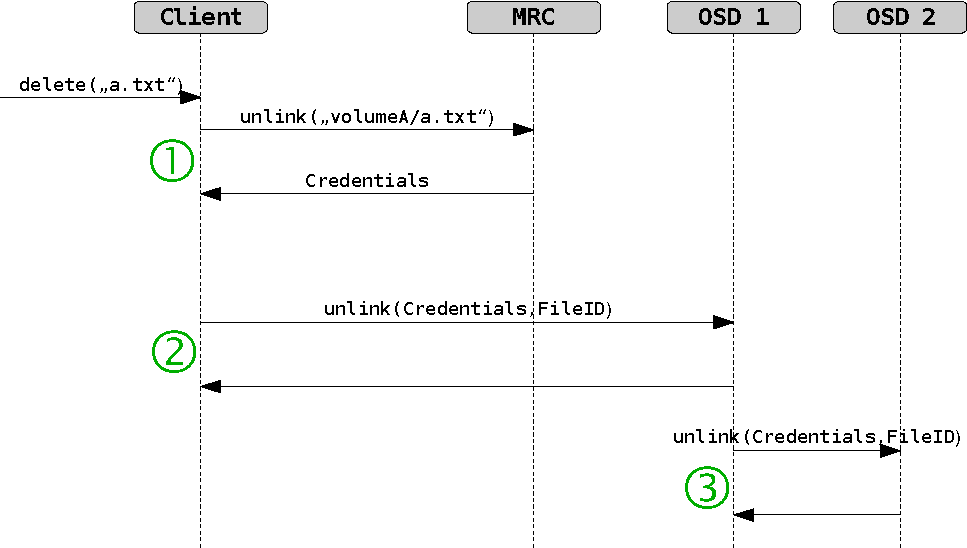
\includegraphics{images/interactions_delete.pdf}}
\caption{Deleting a file}
\label{fig:interactions_delete}
\end{figure}

\paragraph{read}

Files are read as described in the following (see Fig.\ \ref{fig:interactions_read}):

\begin{enumerate}
 \item The client receives an \texttt{open} request from the VFS. It opens the file on the MRC\index{MRC} for reading, and receives the file credentials, which contain the globally unique XtreemFS fileID, a read capability and the replica locations list.
 \item The client sends a request for reading Y bytes of data from the offset Z of the file identified by the fileID. The OSD\index{OSD} returns a buffer containing object data, as well as additional information like checksum failure notifications or padding flags.
 \item If multiple read requests are send, the client has to ensure that the capability is renewed before it times out, in order to keep the file open.
 \item The client reads more data from the file, e.g.\ another object.
 \item The client receives a \texttt{close} call. There is no need to explicitly close the file on the servers; this is implicitly done when the capabilities in the OSD\index{OSD} cache time out.
\end{enumerate}

\begin{figure}[h!]
\centering
\resizebox{0.8\width}{0.8\height}{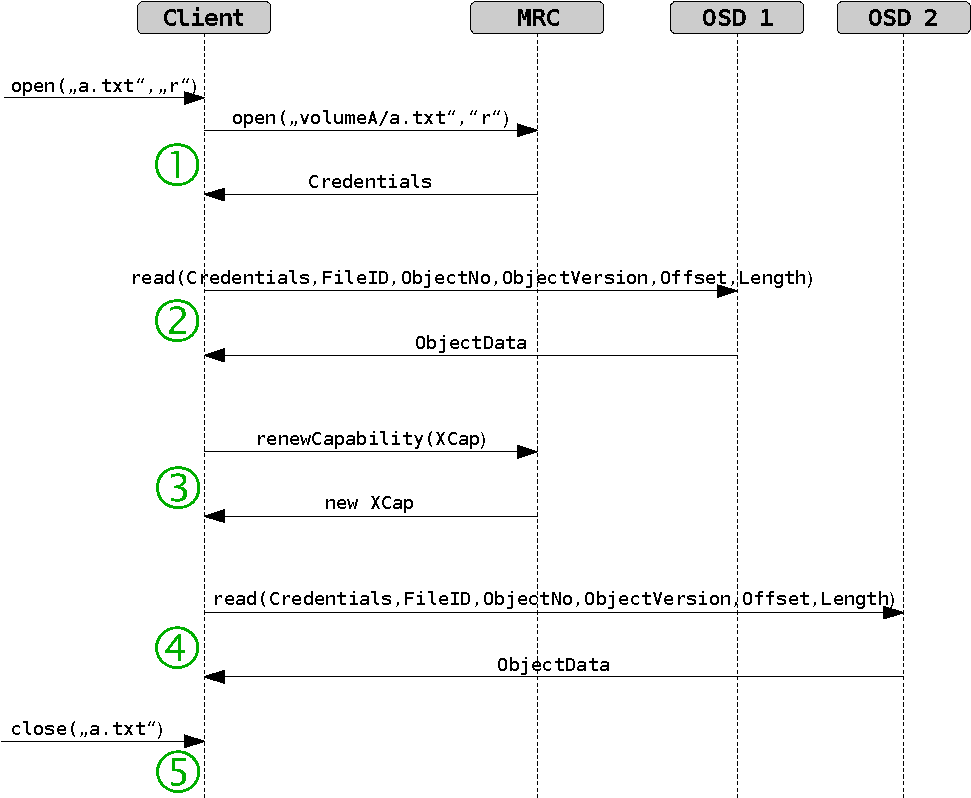
\includegraphics{images/interactions_read.pdf}}
\caption{Reading a file}
\label{fig:interactions_read}
\end{figure}

\paragraph{write}

Files are written as described in the following (see Fig.\ \ref{fig:interactions_write}):

\begin{enumerate}
 \item The client receives an \texttt{open} request from the VFS. It opens the file on the MRC\index{MRC} for writing, and receives the file credentials, which contain the globally unique XtreemFS fileID, a write capability and the replica locations list.
 \item The client sends a buffer containing the data to the OSD\index{OSD} on which the object is stored. In return, the OSD\index{OSD} sends an \texttt{OSDWriteResponse}, which must be cached and sent to the MRC\index{MRC} when the file is closed or fsync is called. The client can also decide to send pending filesize updates from time to time between capability renewals, as the lifetime of a capability can be in the range of tens of minutes.
 \item If multiple write requests are send, the client has to ensure that the capability is renewed before it times out, in order to keep the file open.
 \item The client appends data to the file by sending more \texttt{write} requests, each being answered with an \texttt{OSDWriteResponse}.
 \item The client receives a \texttt{close} call. It sends any pending \texttt{OSDWriteResponse}s to the MRC\index{MRC}, in order to update the file size. There is no need to explicitly close the file on the servers; this is implicitly done when the capabilities in the OSD\index{OSD} cache time out.
\end{enumerate}

\begin{figure}[h!]
\centering
\resizebox{0.8\width}{0.8\height}{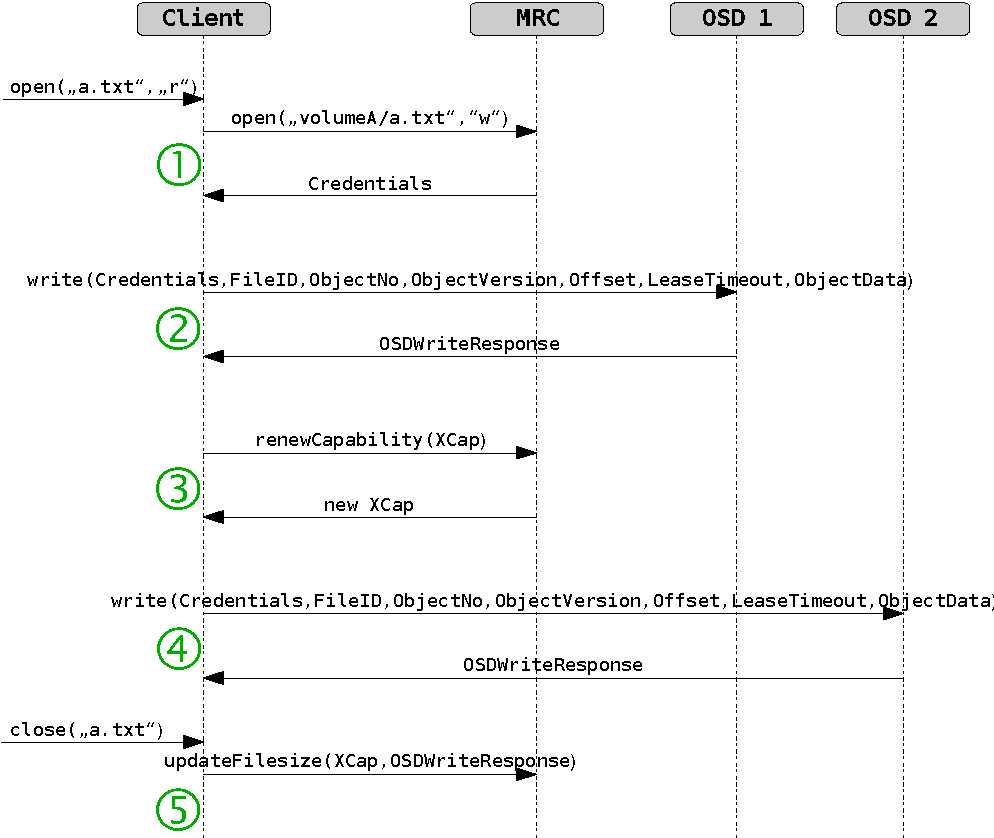
\includegraphics{images/interactions_write.pdf}}
\caption{Writing a file}
\label{fig:interactions_write}
\end{figure}

\paragraph{fsync}

Files are fsync'ed as described in the following (see Fig.\ \ref{fig:interactions_fsync}):

\begin{enumerate}
 \item The file was opened and modified.
 \item The client receives a \texttt{fsync} request from the VFS. If the file is opened all pending data will be written to the OSD\index{OSD}.
 \item The client sends any pending \texttt{OSDWriteResponse}s to the MRC\index{MRC}, in order to update the file size.
 \item The file is further modified or closed.
\end{enumerate}

\begin{figure}[h!]
\centering
\resizebox{0.8\width}{0.8\height}{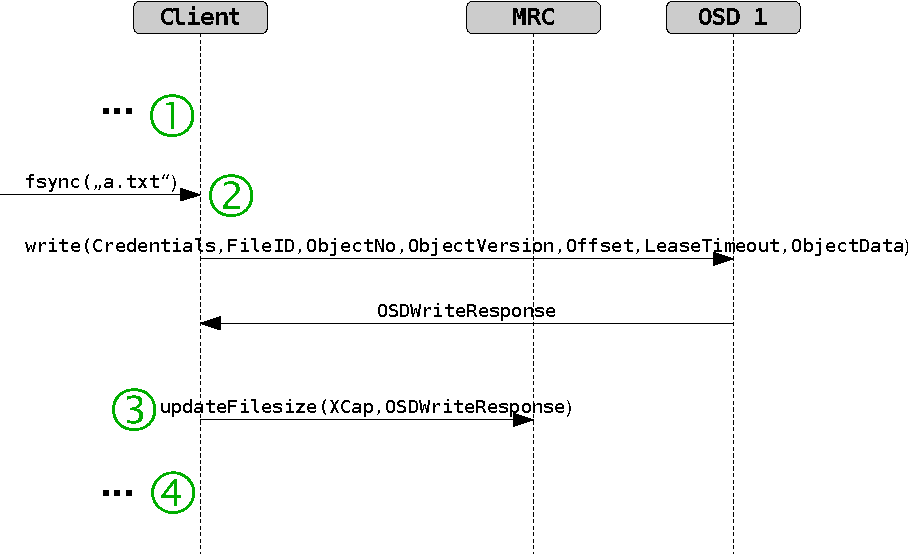
\includegraphics{images/interactions_fsync.pdf}}
\caption{Synchronizing data with the underlying device}
\label{fig:interactions_fsync}
\end{figure}

\paragraph{mkvol}

New volumes are created as described in the following (see Fig.\ \ref{fig:interactions_mkvol}):

\begin{enumerate}
 \item The client receives an \texttt{mkvol} request. In response, it creates the volume on the MRC\index{MRC}.
 \item The MRC\index{MRC} registers the volume at the DIR\index{DIR}.
 \item If no problems occur, the MRC\index{MRC} responds to the client with an acknowledgment.
\end{enumerate}

\begin{figure}[h!]
\centering
\resizebox{0.8\width}{0.8\height}{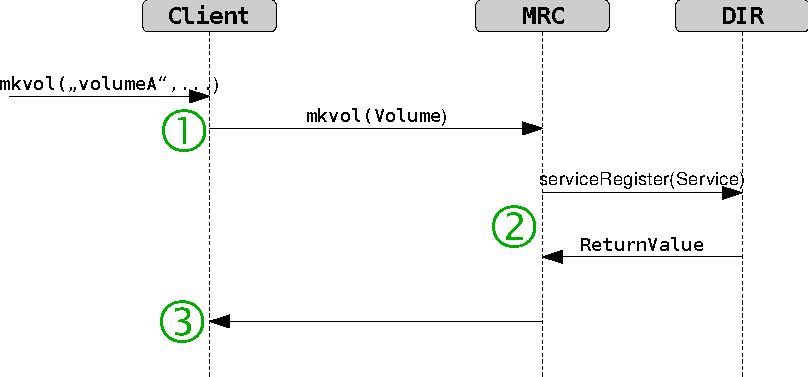
\includegraphics{images/interactions_mkvol.pdf}}
\caption{Creating a new volume}
\label{fig:interactions_mkvol}
\end{figure}

\paragraph{rmvol}

Volumes are deleted as described in the following (see Fig.\ \ref{fig:interactions_rmvol}):

\begin{enumerate}
 \item The client receives a \texttt{rmvol} request from the console. In response, it removes the volume on the MRC\index{MRC}.
 \item The MRC\index{MRC} deregisters the volume at the DIR\index{DIR}.
 \item If no problems occur, the MRC\index{MRC} responds to the client with an acknowledgment.
\end{enumerate}

\begin{figure}[h!]
\centering
\resizebox{0.8\width}{0.8\height}{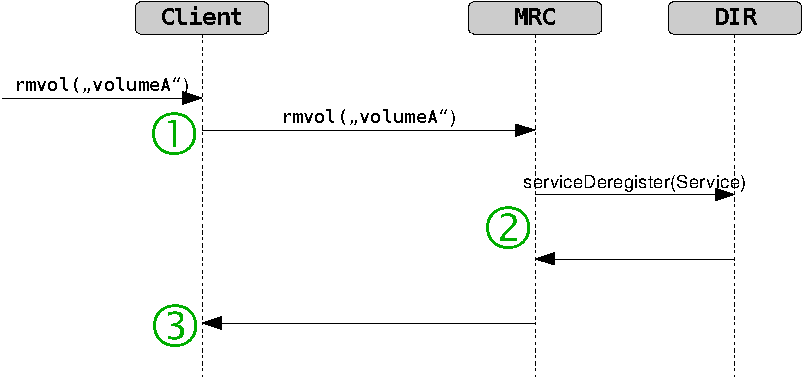
\includegraphics{images/interactions_rmvol.pdf}}
\caption{Deleting an existing volume}
\label{fig:interactions_rmvol}
\end{figure}

\paragraph{removeReplica}

Single replicas of a file are deleted as described in the following (see Fig.\ \ref{fig:interactions_rmrepl}):

\begin{enumerate}
 \item The client receives a \texttt{removeReplica} request from the console. It sends a request to the MRC\index{MRC} to remove the replica with a matching head OSD\index{OSD}. In response, it receives the file credentials, which contain the globally unique XtreemFS fileID, a deletion capability and the list of replica locations.
 \item The client initiates the deletion of the replica's file content by invoking the \texttt{unlink} operation on the head OSD\index{OSD} (i.e.\ the first OSD\index{OSD} of a stripe).
 \item The head OSD\index{OSD} delays the deletion until all clients have closed the file, i.e.\ all capabilities known to the head OSD\index{OSD} have timed out. In turn, the head OSD\index{OSD} initiates the deletion of file objects on the remaining OSDs via \texttt{unlink}.
 \item If a client finds out that its replica locations list for the file is outdated, it has to retrieve the new replica locations list from the MRC\index{MRC}.
\end{enumerate}

\begin{figure}[h!]
\centering
\resizebox{0.8\width}{0.8\height}{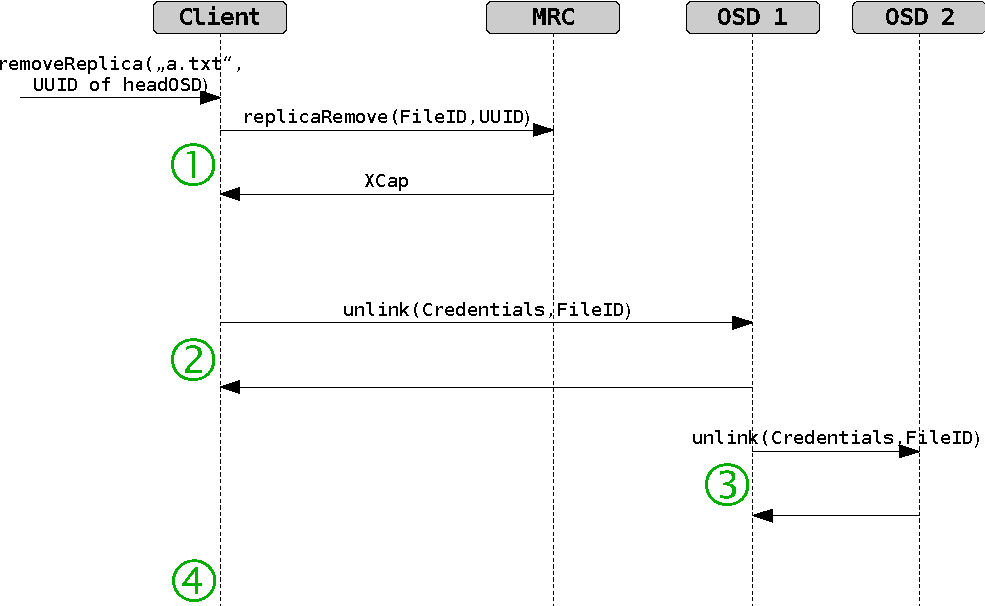
\includegraphics{images/interactions_rmrepl.pdf}}
\caption{Deleting a replica of a file}
\label{fig:interactions_rmrepl}
\end{figure}